\documentclass[1p]{elsarticle_modified}
%\bibliographystyle{elsarticle-num}

%\usepackage[colorlinks]{hyperref}
%\usepackage{abbrmath_seonhwa} %\Abb, \Ascr, \Acal ,\Abf, \Afrak
\usepackage{amsfonts}
\usepackage{amssymb}
\usepackage{amsmath}
\usepackage{amsthm}
\usepackage{scalefnt}
\usepackage{amsbsy}
\usepackage{kotex}
\usepackage{caption}
\usepackage{subfig}
\usepackage{color}
\usepackage{graphicx}
\usepackage{xcolor} %% white, black, red, green, blue, cyan, magenta, yellow
\usepackage{float}
\usepackage{setspace}
\usepackage{hyperref}

\usepackage{tikz}
\usetikzlibrary{arrows}

\usepackage{multirow}
\usepackage{array} % fixed length table
\usepackage{hhline}

%%%%%%%%%%%%%%%%%%%%%
\makeatletter
\renewcommand*\env@matrix[1][\arraystretch]{%
	\edef\arraystretch{#1}%
	\hskip -\arraycolsep
	\let\@ifnextchar\new@ifnextchar
	\array{*\c@MaxMatrixCols c}}
\makeatother %https://tex.stackexchange.com/questions/14071/how-can-i-increase-the-line-spacing-in-a-matrix
%%%%%%%%%%%%%%%

\usepackage[normalem]{ulem}

\newcommand{\msout}[1]{\ifmmode\text{\sout{\ensuremath{#1}}}\else\sout{#1}\fi}
%SOURCE: \msout is \stkout macro in https://tex.stackexchange.com/questions/20609/strikeout-in-math-mode

\newcommand{\cancel}[1]{
	\ifmmode
	{\color{red}\msout{#1}}
	\else
	{\color{red}\sout{#1}}
	\fi
}

\newcommand{\add}[1]{
	{\color{blue}\uwave{#1}}
}

\newcommand{\replace}[2]{
	\ifmmode
	{\color{red}\msout{#1}}{\color{blue}\uwave{#2}}
	\else
	{\color{red}\sout{#1}}{\color{blue}\uwave{#2}}
	\fi
}

\newcommand{\Sol}{\mathcal{S}} %segment
\newcommand{\D}{D} %diagram
\newcommand{\A}{\mathcal{A}} %arc


%%%%%%%%%%%%%%%%%%%%%%%%%%%%%5 test

\def\sl{\operatorname{\textup{SL}}(2,\Cbb)}
\def\psl{\operatorname{\textup{PSL}}(2,\Cbb)}
\def\quan{\mkern 1mu \triangleright \mkern 1mu}

\theoremstyle{definition}
\newtheorem{thm}{Theorem}[section]
\newtheorem{prop}[thm]{Proposition}
\newtheorem{lem}[thm]{Lemma}
\newtheorem{ques}[thm]{Question}
\newtheorem{cor}[thm]{Corollary}
\newtheorem{defn}[thm]{Definition}
\newtheorem{exam}[thm]{Example}
\newtheorem{rmk}[thm]{Remark}
\newtheorem{alg}[thm]{Algorithm}

\newcommand{\I}{\sqrt{-1}}
\begin{document}

%\begin{frontmatter}
%
%\title{Boundary parabolic representations of knots up to 8 crossings}
%
%%% Group authors per affiliation:
%\author{Yunhi Cho} 
%\address{Department of Mathematics, University of Seoul, Seoul, Korea}
%\ead{yhcho@uos.ac.kr}
%
%
%\author{Seonhwa Kim} %\fnref{s_kim}}
%\address{Center for Geometry and Physics, Institute for Basic Science, Pohang, 37673, Korea}
%\ead{ryeona17@ibs.re.kr}
%
%\author{Hyuk Kim}
%\address{Department of Mathematical Sciences, Seoul National University, Seoul 08826, Korea}
%\ead{hyukkim@snu.ac.kr}
%
%\author{Seokbeom Yoon}
%\address{Department of Mathematical Sciences, Seoul National University, Seoul, 08826,  Korea}
%\ead{sbyoon15@snu.ac.kr}
%
%\begin{abstract}
%We find all boundary parabolic representation of knots up to 8 crossings.
%
%\end{abstract}
%\begin{keyword}
%    \MSC[2010] 57M25 
%\end{keyword}
%
%\end{frontmatter}

%\linenumbers
%\tableofcontents
%
\newcommand\colored[1]{\textcolor{white}{\rule[-0.35ex]{0.8em}{1.4ex}}\kern-0.8em\color{red} #1}%
%\newcommand\colored[1]{\textcolor{white}{ #1}\kern-2.17ex	\textcolor{white}{ #1}\kern-1.81ex	\textcolor{white}{ #1}\kern-2.15ex\color{red}#1	}

{\Large $\underline{12a_{0988}~(K12a_{0988})}$}

\setlength{\tabcolsep}{10pt}
\renewcommand{\arraystretch}{1.6}
\vspace{1cm}\begin{tabular}{m{100pt}>{\centering\arraybackslash}m{274pt}}
\multirow{5}{120pt}{
	\centering
	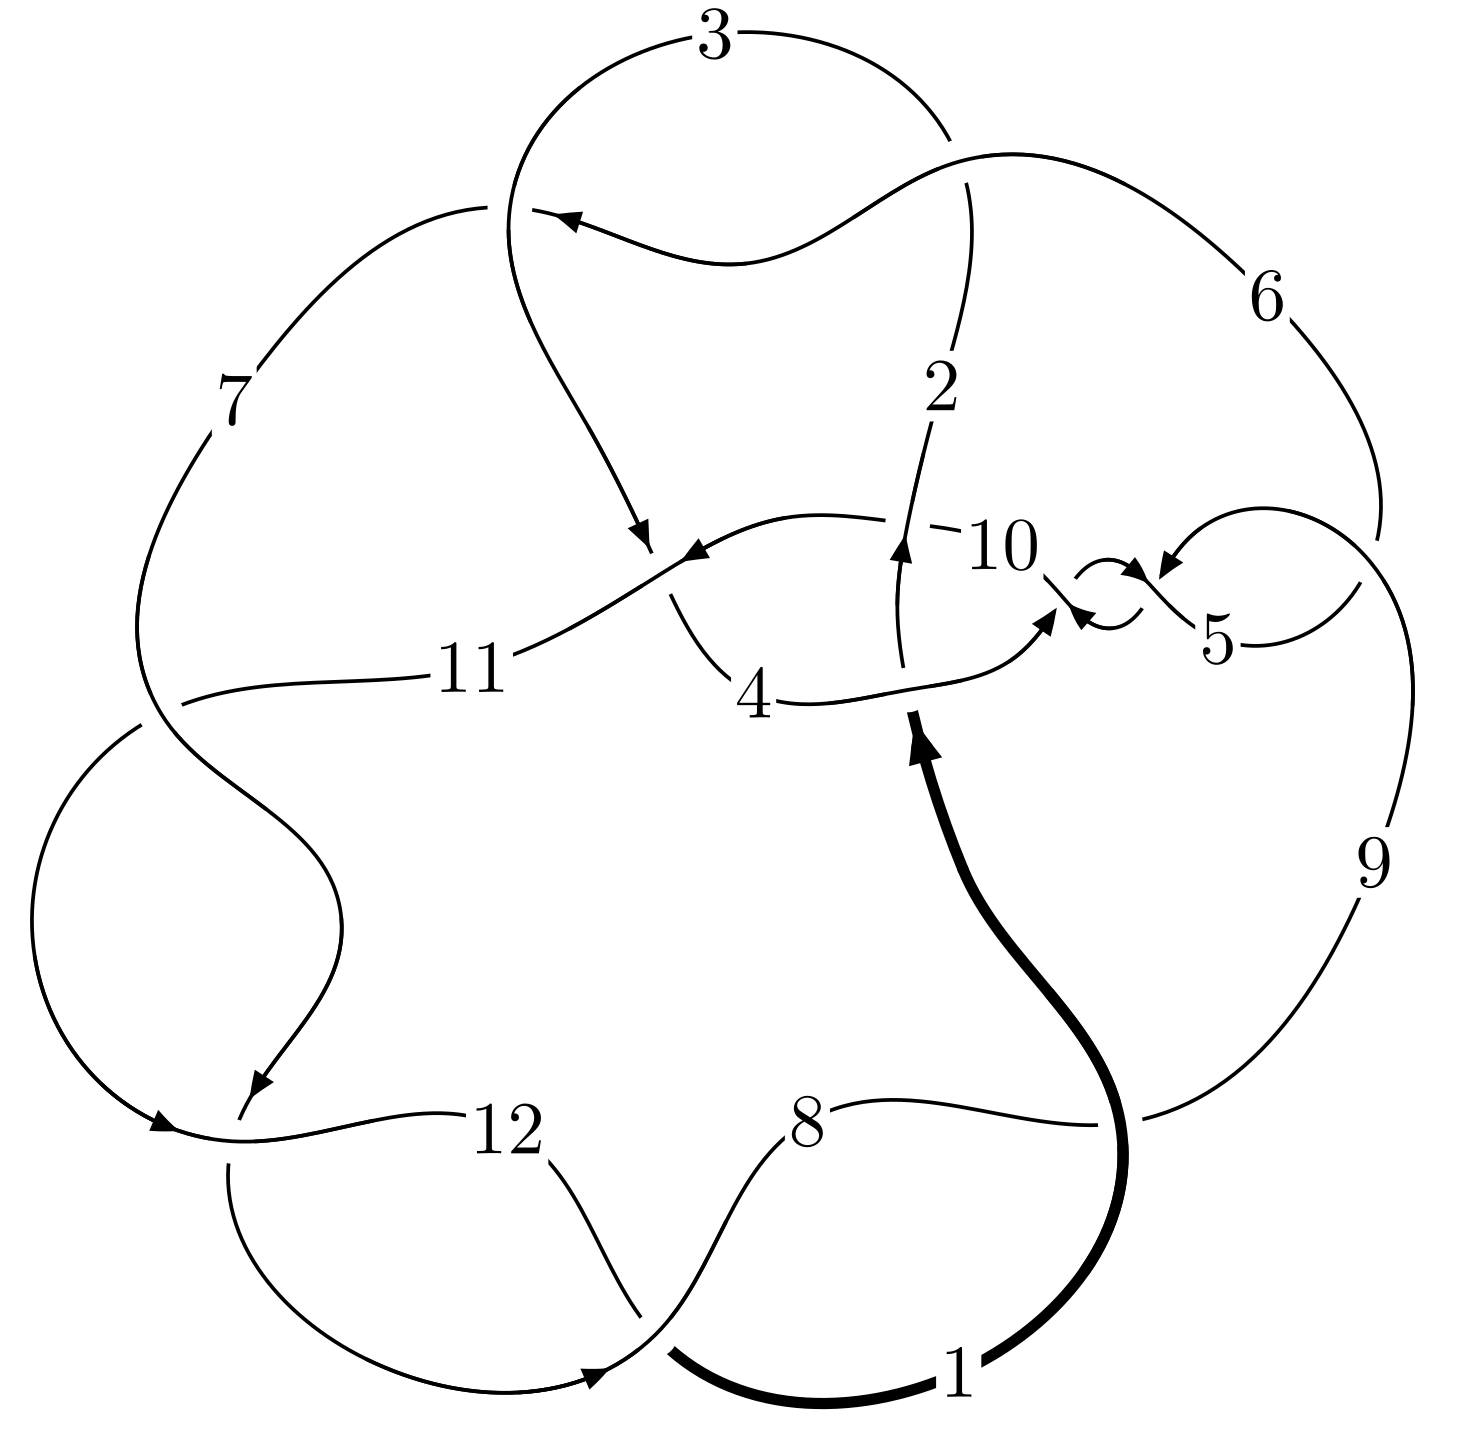
\includegraphics[width=112pt]{../../../GIT/diagram.site/Diagrams/png/1789_12a_0988.png}\\
\ \ \ A knot diagram\footnotemark}&
\allowdisplaybreaks
\textbf{Linearized knot diagam} \\
\cline{2-2}
 &
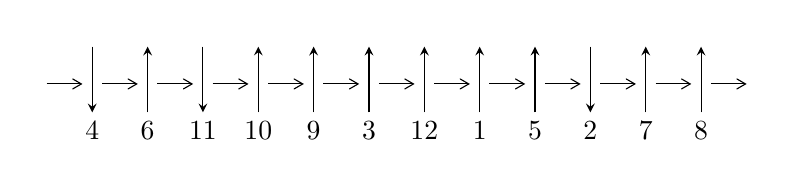
\begin{tikzpicture}[x=20pt, y=17pt]
	% nodes
	\node (C0) at (0, 0) {};
	\node (C1) at (1, 0) {};
	\node (C1U) at (1, +1) {};
	\node (C1D) at (1, -1) {4};

	\node (C2) at (2, 0) {};
	\node (C2U) at (2, +1) {};
	\node (C2D) at (2, -1) {6};

	\node (C3) at (3, 0) {};
	\node (C3U) at (3, +1) {};
	\node (C3D) at (3, -1) {11};

	\node (C4) at (4, 0) {};
	\node (C4U) at (4, +1) {};
	\node (C4D) at (4, -1) {10};

	\node (C5) at (5, 0) {};
	\node (C5U) at (5, +1) {};
	\node (C5D) at (5, -1) {9};

	\node (C6) at (6, 0) {};
	\node (C6U) at (6, +1) {};
	\node (C6D) at (6, -1) {3};

	\node (C7) at (7, 0) {};
	\node (C7U) at (7, +1) {};
	\node (C7D) at (7, -1) {12};

	\node (C8) at (8, 0) {};
	\node (C8U) at (8, +1) {};
	\node (C8D) at (8, -1) {1};

	\node (C9) at (9, 0) {};
	\node (C9U) at (9, +1) {};
	\node (C9D) at (9, -1) {5};

	\node (C10) at (10, 0) {};
	\node (C10U) at (10, +1) {};
	\node (C10D) at (10, -1) {2};

	\node (C11) at (11, 0) {};
	\node (C11U) at (11, +1) {};
	\node (C11D) at (11, -1) {7};

	\node (C12) at (12, 0) {};
	\node (C12U) at (12, +1) {};
	\node (C12D) at (12, -1) {8};
	\node (C13) at (13, 0) {};

	% arrows
	\draw[->,>={angle 60}]
	(C0) edge (C1) (C1) edge (C2) (C2) edge (C3) (C3) edge (C4) (C4) edge (C5) (C5) edge (C6) (C6) edge (C7) (C7) edge (C8) (C8) edge (C9) (C9) edge (C10) (C10) edge (C11) (C11) edge (C12) (C12) edge (C13) ;	\draw[->,>=stealth]
	(C1U) edge (C1D) (C2D) edge (C2U) (C3U) edge (C3D) (C4D) edge (C4U) (C5D) edge (C5U) (C6D) edge (C6U) (C7D) edge (C7U) (C8D) edge (C8U) (C9D) edge (C9U) (C10U) edge (C10D) (C11D) edge (C11U) (C12D) edge (C12U) ;
	\end{tikzpicture} \\
\hhline{~~} \\& 
\textbf{Solving Sequence} \\ \cline{2-2} 
 &
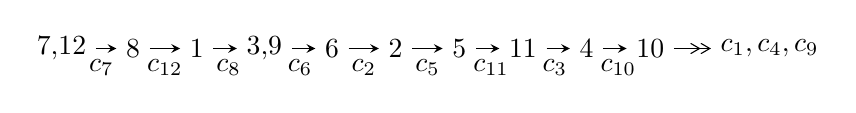
\begin{tikzpicture}[x=23pt, y=7pt]
	% node
	\node (A0) at (-1/8, 0) {7,12};
	\node (A1) at (1, 0) {8};
	\node (A2) at (2, 0) {1};
	\node (A3) at (49/16, 0) {3,9};
	\node (A4) at (33/8, 0) {6};
	\node (A5) at (41/8, 0) {2};
	\node (A6) at (49/8, 0) {5};
	\node (A7) at (57/8, 0) {11};
	\node (A8) at (65/8, 0) {4};
	\node (A9) at (73/8, 0) {10};
	\node (C1) at (1/2, -1) {$c_{7}$};
	\node (C2) at (3/2, -1) {$c_{12}$};
	\node (C3) at (5/2, -1) {$c_{8}$};
	\node (C4) at (29/8, -1) {$c_{6}$};
	\node (C5) at (37/8, -1) {$c_{2}$};
	\node (C6) at (45/8, -1) {$c_{5}$};
	\node (C7) at (53/8, -1) {$c_{11}$};
	\node (C8) at (61/8, -1) {$c_{3}$};
	\node (C9) at (69/8, -1) {$c_{10}$};
	\node (A10) at (11, 0) {$c_{1},c_{4},c_{9}$};

	% edge
	\draw[->,>=stealth]	
	(A0) edge (A1) (A1) edge (A2) (A2) edge (A3) (A3) edge (A4) (A4) edge (A5) (A5) edge (A6) (A6) edge (A7) (A7) edge (A8) (A8) edge (A9) ;
	\draw[->>,>={angle 60}]	
	(A9) edge (A10);
\end{tikzpicture} \\ 

\end{tabular} \\

\footnotetext{
The image of knot diagram is generated by the software ``\textbf{Draw programme}" developed by Andrew Bartholomew(\url{http://www.layer8.co.uk/maths/draw/index.htm\#Running-draw}), where we modified some parts for our purpose(\url{https://github.com/CATsTAILs/LinksPainter}).
}\phantom \\ \newline 
\centering \textbf{Ideals for irreducible components\footnotemark of $X_{\text{par}}$} 
 
\begin{align*}
I^u_{1}&=\langle 
-1.41244\times10^{69} u^{68}-3.32508\times10^{69} u^{67}+\cdots+3.39317\times10^{69} b+1.80676\times10^{70},\\
\phantom{I^u_{1}}&\phantom{= \langle  }1.05888\times10^{70} u^{68}+2.32754\times10^{70} u^{67}+\cdots+2.37522\times10^{70} a-1.91976\times10^{71},\\
\phantom{I^u_{1}}&\phantom{= \langle  }u^{69}+4 u^{68}+\cdots+118 u-28\rangle \\
I^u_{2}&=\langle 
- u^3+b+2 u,\;u^{16}- u^{15}+\cdots+a-2,\;u^{17}-12 u^{15}+\cdots+10 u^2-1\rangle \\
I^u_{3}&=\langle 
-186 a^4 u-87 a^4-392 a^3 u-230 a^3+1248 a^2 u+506 a^2+2922 a u+241 b+1289 a+282 u-78,\\
\phantom{I^u_{3}}&\phantom{= \langle  }a^5+2 a^4+a^3 u-8 a^3+10 a^2 u-30 a^2+17 a u-29 a+8 u-13,\;u^2- u-1\rangle \\
\\
\end{align*}
\raggedright * 3 irreducible components of $\dim_{\mathbb{C}}=0$, with total 96 representations.\\
\footnotetext{All coefficients of polynomials are rational numbers. But the coefficients are sometimes approximated in decimal forms when there is not enough margin.}
\newpage
\renewcommand{\arraystretch}{1}
\centering \section*{I. $I^u_{1}= \langle -1.41\times10^{69} u^{68}-3.33\times10^{69} u^{67}+\cdots+3.39\times10^{69} b+1.81\times10^{70},\;1.06\times10^{70} u^{68}+2.33\times10^{70} u^{67}+\cdots+2.38\times10^{70} a-1.92\times10^{71},\;u^{69}+4 u^{68}+\cdots+118 u-28 \rangle$}
\flushleft \textbf{(i) Arc colorings}\\
\begin{tabular}{m{7pt} m{180pt} m{7pt} m{180pt} }
\flushright $a_{7}=$&$\begin{pmatrix}1\\0\end{pmatrix}$ \\
\flushright $a_{12}=$&$\begin{pmatrix}0\\u\end{pmatrix}$ \\
\flushright $a_{8}=$&$\begin{pmatrix}1\\- u^2\end{pmatrix}$ \\
\flushright $a_{1}=$&$\begin{pmatrix}u\\- u^3+u\end{pmatrix}$ \\
\flushright $a_{3}=$&$\begin{pmatrix}-0.445803 u^{68}-0.979926 u^{67}+\cdots-37.8294 u+8.08246\\0.416260 u^{68}+0.979934 u^{67}+\cdots+31.7679 u-5.32469\end{pmatrix}$ \\
\flushright $a_{9}=$&$\begin{pmatrix}- u^2+1\\u^4-2 u^2\end{pmatrix}$ \\
\flushright $a_{6}=$&$\begin{pmatrix}-0.337813 u^{68}-0.689657 u^{67}+\cdots-32.8264 u+7.20315\\0.182878 u^{68}+0.451924 u^{67}+\cdots+7.26000 u-0.225713\end{pmatrix}$ \\
\flushright $a_{2}=$&$\begin{pmatrix}-0.279350 u^{68}-0.735303 u^{67}+\cdots-17.4605 u+4.28483\\0.356355 u^{68}+0.862570 u^{67}+\cdots+35.2557 u-6.44200\end{pmatrix}$ \\
\flushright $a_{5}=$&$\begin{pmatrix}0.864573 u^{68}+2.07589 u^{67}+\cdots+74.2680 u-16.1219\\-1.15159 u^{68}-2.66334 u^{67}+\cdots-108.556 u+24.4015\end{pmatrix}$ \\
\flushright $a_{11}=$&$\begin{pmatrix}- u\\u\end{pmatrix}$ \\
\flushright $a_{4}=$&$\begin{pmatrix}-0.201645 u^{68}-0.481748 u^{67}+\cdots-23.0572 u+4.77346\\0.172103 u^{68}+0.481755 u^{67}+\cdots+16.9956 u-2.01569\end{pmatrix}$ \\
\flushright $a_{10}=$&$\begin{pmatrix}0.878887 u^{68}+2.21773 u^{67}+\cdots+57.9452 u-9.67980\\-0.809320 u^{68}-1.99188 u^{67}+\cdots-55.2577 u+11.7419\end{pmatrix}$\\&\end{tabular}
\flushleft \textbf{(ii) Obstruction class $= -1$}\\~\\
\flushleft \textbf{(iii) Cusp Shapes $= -0.841314 u^{68}-1.63044 u^{67}+\cdots-102.614 u+28.7772$}\\~\\
\newpage\renewcommand{\arraystretch}{1}
\flushleft \textbf{(iv) u-Polynomials at the component}\newline \\
\begin{tabular}{m{50pt}|m{274pt}}
Crossings & \hspace{64pt}u-Polynomials at each crossing \\
\hline $$\begin{aligned}c_{1}\end{aligned}$$&$\begin{aligned}
&u^{69}-9 u^{68}+\cdots-125 u-1
\end{aligned}$\\
\hline $$\begin{aligned}c_{2},c_{6}\end{aligned}$$&$\begin{aligned}
&u^{69}-4 u^{68}+\cdots+1186 u+1279
\end{aligned}$\\
\hline $$\begin{aligned}c_{3}\end{aligned}$$&$\begin{aligned}
&u^{69}+19 u^{67}+\cdots-73191 u+47449
\end{aligned}$\\
\hline $$\begin{aligned}c_{4},c_{5},c_{9}\end{aligned}$$&$\begin{aligned}
&u^{69}-2 u^{68}+\cdots-82 u+1
\end{aligned}$\\
\hline $$\begin{aligned}c_{7},c_{8},c_{11}\\c_{12}\end{aligned}$$&$\begin{aligned}
&u^{69}-4 u^{68}+\cdots+118 u+28
\end{aligned}$\\
\hline $$\begin{aligned}c_{10}\end{aligned}$$&$\begin{aligned}
&u^{69}+4 u^{68}+\cdots+171 u-29
\end{aligned}$\\
\hline
\end{tabular}\\~\\
\newpage\renewcommand{\arraystretch}{1}
\flushleft \textbf{(v) Riley Polynomials at the component}\newline \\
\begin{tabular}{m{50pt}|m{274pt}}
Crossings & \hspace{64pt}Riley Polynomials at each crossing \\
\hline $$\begin{aligned}c_{1}\end{aligned}$$&$\begin{aligned}
&y^{69}+9 y^{68}+\cdots+17785 y-1
\end{aligned}$\\
\hline $$\begin{aligned}c_{2},c_{6}\end{aligned}$$&$\begin{aligned}
&y^{69}-52 y^{68}+\cdots+50080220 y-1635841
\end{aligned}$\\
\hline $$\begin{aligned}c_{3}\end{aligned}$$&$\begin{aligned}
&y^{69}+38 y^{68}+\cdots-35937183035 y-2251407601
\end{aligned}$\\
\hline $$\begin{aligned}c_{4},c_{5},c_{9}\end{aligned}$$&$\begin{aligned}
&y^{69}+70 y^{68}+\cdots+6500 y-1
\end{aligned}$\\
\hline $$\begin{aligned}c_{7},c_{8},c_{11}\\c_{12}\end{aligned}$$&$\begin{aligned}
&y^{69}-84 y^{68}+\cdots+6364 y-784
\end{aligned}$\\
\hline $$\begin{aligned}c_{10}\end{aligned}$$&$\begin{aligned}
&y^{69}-14 y^{68}+\cdots+39333 y-841
\end{aligned}$\\
\hline
\end{tabular}\\~\\
\newpage\flushleft \textbf{(vi) Complex Volumes and Cusp Shapes}
$$\begin{array}{c|c|c}  
\text{Solutions to }I^u_{1}& \I (\text{vol} + \sqrt{-1}CS) & \text{Cusp shape}\\
 \hline 
\begin{aligned}
u &= \phantom{-}0.885057 + 0.508714 I \\
a &= -1.25938 + 1.09741 I \\
b &= \phantom{-}1.313650 + 0.417375 I\end{aligned}
 & \phantom{-}5.12644 + 8.14034 I & \phantom{-0.000000 } 0 \\ \hline\begin{aligned}
u &= \phantom{-}0.885057 - 0.508714 I \\
a &= -1.25938 - 1.09741 I \\
b &= \phantom{-}1.313650 - 0.417375 I\end{aligned}
 & \phantom{-}5.12644 - 8.14034 I & \phantom{-0.000000 } 0 \\ \hline\begin{aligned}
u &= -1.016630 + 0.148616 I \\
a &= -1.354710 - 0.051330 I \\
b &= \phantom{-}1.152720 - 0.802920 I\end{aligned}
 & \phantom{-}0.08436 - 3.60660 I & \phantom{-0.000000 } 0 \\ \hline\begin{aligned}
u &= -1.016630 - 0.148616 I \\
a &= -1.354710 + 0.051330 I \\
b &= \phantom{-}1.152720 + 0.802920 I\end{aligned}
 & \phantom{-}0.08436 + 3.60660 I & \phantom{-0.000000 } 0 \\ \hline\begin{aligned}
u &= \phantom{-}0.636042 + 0.735204 I \\
a &= \phantom{-}0.771040 - 0.820398 I \\
b &= -1.385970 - 0.048806 I\end{aligned}
 & \phantom{-}1.71288 + 2.51836 I & \phantom{-0.000000 } 0 \\ \hline\begin{aligned}
u &= \phantom{-}0.636042 - 0.735204 I \\
a &= \phantom{-}0.771040 + 0.820398 I \\
b &= -1.385970 + 0.048806 I\end{aligned}
 & \phantom{-}1.71288 - 2.51836 I & \phantom{-0.000000 } 0 \\ \hline\begin{aligned}
u &= -0.896655 + 0.578537 I \\
a &= -0.888310 - 0.824652 I \\
b &= \phantom{-}1.234820 + 0.008364 I\end{aligned}
 & \phantom{-}4.86851 - 0.44171 I & \phantom{-0.000000 } 0 \\ \hline\begin{aligned}
u &= -0.896655 - 0.578537 I \\
a &= -0.888310 + 0.824652 I \\
b &= \phantom{-}1.234820 - 0.008364 I\end{aligned}
 & \phantom{-}4.86851 + 0.44171 I & \phantom{-0.000000 } 0 \\ \hline\begin{aligned}
u &= -0.906672 + 0.619011 I \\
a &= \phantom{-}1.24005 + 0.82717 I \\
b &= -1.36590 + 0.51916 I\end{aligned}
 & -0.78365 - 12.22400 I & \phantom{-0.000000 } 0 \\ \hline\begin{aligned}
u &= -0.906672 - 0.619011 I \\
a &= \phantom{-}1.24005 - 0.82717 I \\
b &= -1.36590 - 0.51916 I\end{aligned}
 & -0.78365 + 12.22400 I & \phantom{-0.000000 } 0\\
 \hline 
 \end{array}$$\newpage$$\begin{array}{c|c|c}  
\text{Solutions to }I^u_{1}& \I (\text{vol} + \sqrt{-1}CS) & \text{Cusp shape}\\
 \hline 
\begin{aligned}
u &= -0.044130 + 0.894273 I \\
a &= \phantom{-}0.0367545 - 0.0279078 I \\
b &= -1.218310 - 0.375774 I\end{aligned}
 & -3.41603 + 7.23977 I & \phantom{-}6.00000 - 5.79158 I \\ \hline\begin{aligned}
u &= -0.044130 - 0.894273 I \\
a &= \phantom{-}0.0367545 + 0.0279078 I \\
b &= -1.218310 + 0.375774 I\end{aligned}
 & -3.41603 - 7.23977 I & \phantom{-}6.00000 + 5.79158 I \\ \hline\begin{aligned}
u &= -0.769410 + 0.383812 I \\
a &= \phantom{-}1.04791 + 1.63891 I \\
b &= -1.180600 + 0.315893 I\end{aligned}
 & \phantom{-}3.85880 - 3.01933 I & \phantom{-}9.96983 + 6.07662 I \\ \hline\begin{aligned}
u &= -0.769410 - 0.383812 I \\
a &= \phantom{-}1.04791 - 1.63891 I \\
b &= -1.180600 - 0.315893 I\end{aligned}
 & \phantom{-}3.85880 + 3.01933 I & \phantom{-}9.96983 - 6.07662 I \\ \hline\begin{aligned}
u &= \phantom{-}0.836904 + 0.153168 I \\
a &= \phantom{-}1.49560 - 0.59674 I \\
b &= -1.343630 - 0.417966 I\end{aligned}
 & \phantom{-}4.62859 + 1.66065 I & \phantom{-}18.4070 - 5.0043 I \\ \hline\begin{aligned}
u &= \phantom{-}0.836904 - 0.153168 I \\
a &= \phantom{-}1.49560 + 0.59674 I \\
b &= -1.343630 + 0.417966 I\end{aligned}
 & \phantom{-}4.62859 - 1.66065 I & \phantom{-}18.4070 + 5.0043 I \\ \hline\begin{aligned}
u &= -0.709314 + 0.400333 I \\
a &= -0.178614 + 0.107335 I \\
b &= -0.011683 - 1.196020 I\end{aligned}
 & -5.11512 - 6.32617 I & \phantom{-}4.96847 + 7.99574 I \\ \hline\begin{aligned}
u &= -0.709314 - 0.400333 I \\
a &= -0.178614 - 0.107335 I \\
b &= -0.011683 + 1.196020 I\end{aligned}
 & -5.11512 + 6.32617 I & \phantom{-}4.96847 - 7.99574 I \\ \hline\begin{aligned}
u &= \phantom{-}0.746120 + 0.270176 I \\
a &= \phantom{-}0.431126 - 0.142662 I \\
b &= -0.078465 - 0.885255 I\end{aligned}
 & \phantom{-}0.83816 + 3.48222 I & \phantom{-}8.75635 - 8.60776 I \\ \hline\begin{aligned}
u &= \phantom{-}0.746120 - 0.270176 I \\
a &= \phantom{-}0.431126 + 0.142662 I \\
b &= -0.078465 + 0.885255 I\end{aligned}
 & \phantom{-}0.83816 - 3.48222 I & \phantom{-}8.75635 + 8.60776 I\\
 \hline 
 \end{array}$$\newpage$$\begin{array}{c|c|c}  
\text{Solutions to }I^u_{1}& \I (\text{vol} + \sqrt{-1}CS) & \text{Cusp shape}\\
 \hline 
\begin{aligned}
u &= -1.22679\phantom{ +0.000000I} \\
a &= -1.24264\phantom{ +0.000000I} \\
b &= \phantom{-}0.596925\phantom{ +0.000000I}\end{aligned}
 & \phantom{-}2.39981\phantom{ +0.000000I} & \phantom{-0.000000 } 0 \\ \hline\begin{aligned}
u &= \phantom{-}0.502427 + 0.575755 I \\
a &= \phantom{-}0.632278 + 0.570820 I \\
b &= \phantom{-}0.593291 - 0.256882 I\end{aligned}
 & -4.44506 + 2.24811 I & \phantom{-}4.48548 - 1.48739 I \\ \hline\begin{aligned}
u &= \phantom{-}0.502427 - 0.575755 I \\
a &= \phantom{-}0.632278 - 0.570820 I \\
b &= \phantom{-}0.593291 + 0.256882 I\end{aligned}
 & -4.44506 - 2.24811 I & \phantom{-}4.48548 + 1.48739 I \\ \hline\begin{aligned}
u &= -0.032139 + 0.742398 I \\
a &= \phantom{-}0.130428 - 0.345678 I \\
b &= \phantom{-}1.211830 - 0.239682 I\end{aligned}
 & \phantom{-}2.35512 - 3.98609 I & \phantom{-}9.19250 + 6.28784 I \\ \hline\begin{aligned}
u &= -0.032139 - 0.742398 I \\
a &= \phantom{-}0.130428 + 0.345678 I \\
b &= \phantom{-}1.211830 + 0.239682 I\end{aligned}
 & \phantom{-}2.35512 + 3.98609 I & \phantom{-}9.19250 - 6.28784 I \\ \hline\begin{aligned}
u &= \phantom{-}1.099620 + 0.619020 I \\
a &= \phantom{-}0.808964 - 0.837395 I \\
b &= -1.137280 + 0.162151 I\end{aligned}
 & -0.01258 - 2.07394 I & \phantom{-0.000000 } 0 \\ \hline\begin{aligned}
u &= \phantom{-}1.099620 - 0.619020 I \\
a &= \phantom{-}0.808964 + 0.837395 I \\
b &= -1.137280 - 0.162151 I\end{aligned}
 & -0.01258 + 2.07394 I & \phantom{-0.000000 } 0 \\ \hline\begin{aligned}
u &= \phantom{-}1.263810 + 0.241659 I \\
a &= \phantom{-}1.34299 + 0.51814 I \\
b &= -0.572476 - 0.299994 I\end{aligned}
 & -1.95538 - 0.27990 I & \phantom{-0.000000 } 0 \\ \hline\begin{aligned}
u &= \phantom{-}1.263810 - 0.241659 I \\
a &= \phantom{-}1.34299 - 0.51814 I \\
b &= -0.572476 + 0.299994 I\end{aligned}
 & -1.95538 + 0.27990 I & \phantom{-0.000000 } 0 \\ \hline\begin{aligned}
u &= \phantom{-}0.668449 + 0.182768 I \\
a &= -3.22718 - 0.46140 I \\
b &= \phantom{-}0.943084 + 0.285478 I\end{aligned}
 & -3.62595 + 4.73786 I & \phantom{-}7.87798 - 6.16232 I\\
 \hline 
 \end{array}$$\newpage$$\begin{array}{c|c|c}  
\text{Solutions to }I^u_{1}& \I (\text{vol} + \sqrt{-1}CS) & \text{Cusp shape}\\
 \hline 
\begin{aligned}
u &= \phantom{-}0.668449 - 0.182768 I \\
a &= -3.22718 + 0.46140 I \\
b &= \phantom{-}0.943084 - 0.285478 I\end{aligned}
 & -3.62595 - 4.73786 I & \phantom{-}7.87798 + 6.16232 I \\ \hline\begin{aligned}
u &= \phantom{-}0.412391 + 0.548973 I \\
a &= \phantom{-}0.155129 + 0.716030 I \\
b &= \phantom{-}0.736431 + 0.522225 I\end{aligned}
 & -4.65764 + 1.61626 I & \phantom{-}2.82750 - 4.30956 I \\ \hline\begin{aligned}
u &= \phantom{-}0.412391 - 0.548973 I \\
a &= \phantom{-}0.155129 - 0.716030 I \\
b &= \phantom{-}0.736431 - 0.522225 I\end{aligned}
 & -4.65764 - 1.61626 I & \phantom{-}2.82750 + 4.30956 I \\ \hline\begin{aligned}
u &= -0.219158 + 0.552429 I \\
a &= \phantom{-}1.53288 + 0.30165 I \\
b &= -0.223631 + 0.772688 I\end{aligned}
 & -6.59300 + 3.04852 I & \phantom{-}0.086786 - 0.536752 I \\ \hline\begin{aligned}
u &= -0.219158 - 0.552429 I \\
a &= \phantom{-}1.53288 - 0.30165 I \\
b &= -0.223631 - 0.772688 I\end{aligned}
 & -6.59300 - 3.04852 I & \phantom{-}0.086786 + 0.536752 I \\ \hline\begin{aligned}
u &= \phantom{-}1.49203\phantom{ +0.000000I} \\
a &= -0.152282\phantom{ +0.000000I} \\
b &= -0.616971\phantom{ +0.000000I}\end{aligned}
 & \phantom{-}6.96786\phantom{ +0.000000I} & \phantom{-0.000000 } 0 \\ \hline\begin{aligned}
u &= -1.51224 + 0.16519 I \\
a &= -0.052321 - 0.516958 I \\
b &= \phantom{-}0.511789 + 0.054440 I\end{aligned}
 & \phantom{-}2.17563 - 4.90185 I & \phantom{-0.000000 } 0 \\ \hline\begin{aligned}
u &= -1.51224 - 0.16519 I \\
a &= -0.052321 + 0.516958 I \\
b &= \phantom{-}0.511789 - 0.054440 I\end{aligned}
 & \phantom{-}2.17563 + 4.90185 I & \phantom{-0.000000 } 0 \\ \hline\begin{aligned}
u &= -1.53515 + 0.04841 I \\
a &= -0.797218 - 0.049788 I \\
b &= \phantom{-}0.833772 - 0.898244 I\end{aligned}
 & \phantom{-}1.47969 - 3.26450 I & \phantom{-0.000000 } 0 \\ \hline\begin{aligned}
u &= -1.53515 - 0.04841 I \\
a &= -0.797218 + 0.049788 I \\
b &= \phantom{-}0.833772 + 0.898244 I\end{aligned}
 & \phantom{-}1.47969 + 3.26450 I & \phantom{-0.000000 } 0\\
 \hline 
 \end{array}$$\newpage$$\begin{array}{c|c|c}  
\text{Solutions to }I^u_{1}& \I (\text{vol} + \sqrt{-1}CS) & \text{Cusp shape}\\
 \hline 
\begin{aligned}
u &= -0.089185 + 0.433722 I \\
a &= -1.301320 - 0.439390 I \\
b &= -1.085960 - 0.017290 I\end{aligned}
 & \phantom{-}1.86291 + 0.12476 I & \phantom{-}6.99819 + 0.57622 I \\ \hline\begin{aligned}
u &= -0.089185 - 0.433722 I \\
a &= -1.301320 + 0.439390 I \\
b &= -1.085960 + 0.017290 I\end{aligned}
 & \phantom{-}1.86291 - 0.12476 I & \phantom{-}6.99819 - 0.57622 I \\ \hline\begin{aligned}
u &= \phantom{-}0.068174 + 0.406678 I \\
a &= -1.01773 + 1.10026 I \\
b &= \phantom{-}0.051644 + 0.523892 I\end{aligned}
 & -1.15029 - 1.08308 I & -0.94169 + 2.86009 I \\ \hline\begin{aligned}
u &= \phantom{-}0.068174 - 0.406678 I \\
a &= -1.01773 - 1.10026 I \\
b &= \phantom{-}0.051644 - 0.523892 I\end{aligned}
 & -1.15029 + 1.08308 I & -0.94169 - 2.86009 I \\ \hline\begin{aligned}
u &= -0.410283\phantom{ +0.000000I} \\
a &= -1.01651\phantom{ +0.000000I} \\
b &= -0.420595\phantom{ +0.000000I}\end{aligned}
 & \phantom{-}0.822559\phantom{ +0.000000I} & \phantom{-}13.9630\phantom{ +0.000000I} \\ \hline\begin{aligned}
u &= \phantom{-}0.323738 + 0.194743 I \\
a &= -0.41274 - 1.81065 I \\
b &= \phantom{-}0.838599 - 0.702790 I\end{aligned}
 & -4.62796 - 3.27883 I & \phantom{-}5.32821 - 2.18413 I \\ \hline\begin{aligned}
u &= \phantom{-}0.323738 - 0.194743 I \\
a &= -0.41274 + 1.81065 I \\
b &= \phantom{-}0.838599 + 0.702790 I\end{aligned}
 & -4.62796 + 3.27883 I & \phantom{-}5.32821 + 2.18413 I \\ \hline\begin{aligned}
u &= -1.62231 + 0.04624 I \\
a &= -2.43198 + 0.36370 I \\
b &= \phantom{-}1.173720 - 0.075551 I\end{aligned}
 & \phantom{-}4.39357 - 5.56424 I & \phantom{-0.000000 } 0 \\ \hline\begin{aligned}
u &= -1.62231 - 0.04624 I \\
a &= -2.43198 - 0.36370 I \\
b &= \phantom{-}1.173720 + 0.075551 I\end{aligned}
 & \phantom{-}4.39357 + 5.56424 I & \phantom{-0.000000 } 0 \\ \hline\begin{aligned}
u &= \phantom{-}1.62794 + 0.10132 I \\
a &= -0.214550 - 0.885759 I \\
b &= \phantom{-}0.06305 + 1.51910 I\end{aligned}
 & \phantom{-}2.96097 + 8.14106 I & \phantom{-0.000000 } 0\\
 \hline 
 \end{array}$$\newpage$$\begin{array}{c|c|c}  
\text{Solutions to }I^u_{1}& \I (\text{vol} + \sqrt{-1}CS) & \text{Cusp shape}\\
 \hline 
\begin{aligned}
u &= \phantom{-}1.62794 - 0.10132 I \\
a &= -0.214550 + 0.885759 I \\
b &= \phantom{-}0.06305 - 1.51910 I\end{aligned}
 & \phantom{-}2.96097 - 8.14106 I & \phantom{-0.000000 } 0 \\ \hline\begin{aligned}
u &= -1.63793 + 0.06004 I \\
a &= \phantom{-}0.303364 - 0.514810 I \\
b &= -0.104398 + 1.183180 I\end{aligned}
 & \phantom{-}9.14294 - 4.64744 I & \phantom{-0.000000 } 0 \\ \hline\begin{aligned}
u &= -1.63793 - 0.06004 I \\
a &= \phantom{-}0.303364 + 0.514810 I \\
b &= -0.104398 - 1.183180 I\end{aligned}
 & \phantom{-}9.14294 + 4.64744 I & \phantom{-0.000000 } 0 \\ \hline\begin{aligned}
u &= \phantom{-}1.64036 + 0.11039 I \\
a &= \phantom{-}1.66328 - 0.72027 I \\
b &= -1.267400 - 0.503838 I\end{aligned}
 & \phantom{-}12.18870 + 4.90550 I & \phantom{-0.000000 } 0 \\ \hline\begin{aligned}
u &= \phantom{-}1.64036 - 0.11039 I \\
a &= \phantom{-}1.66328 + 0.72027 I \\
b &= -1.267400 + 0.503838 I\end{aligned}
 & \phantom{-}12.18870 - 4.90550 I & \phantom{-0.000000 } 0 \\ \hline\begin{aligned}
u &= -1.63556 + 0.21597 I \\
a &= \phantom{-}1.85907 + 0.58231 I \\
b &= -1.50689 + 0.15630 I\end{aligned}
 & \phantom{-}9.45657 - 6.06793 I & \phantom{-0.000000 } 0 \\ \hline\begin{aligned}
u &= -1.63556 - 0.21597 I \\
a &= \phantom{-}1.85907 - 0.58231 I \\
b &= -1.50689 - 0.15630 I\end{aligned}
 & \phantom{-}9.45657 + 6.06793 I & \phantom{-0.000000 } 0 \\ \hline\begin{aligned}
u &= -1.66810 + 0.03752 I \\
a &= \phantom{-}1.97899 - 0.02011 I \\
b &= -1.57935 + 0.61268 I\end{aligned}
 & \phantom{-}13.45550 - 2.36434 I & \phantom{-0.000000 } 0 \\ \hline\begin{aligned}
u &= -1.66810 - 0.03752 I \\
a &= \phantom{-}1.97899 + 0.02011 I \\
b &= -1.57935 - 0.61268 I\end{aligned}
 & \phantom{-}13.45550 + 2.36434 I & \phantom{-0.000000 } 0 \\ \hline\begin{aligned}
u &= -1.67186 + 0.14663 I \\
a &= -1.88316 - 0.52112 I \\
b &= \phantom{-}1.42741 - 0.53981 I\end{aligned}
 & \phantom{-}13.9239 - 10.7016 I & \phantom{-0.000000 } 0\\
 \hline 
 \end{array}$$\newpage$$\begin{array}{c|c|c}  
\text{Solutions to }I^u_{1}& \I (\text{vol} + \sqrt{-1}CS) & \text{Cusp shape}\\
 \hline 
\begin{aligned}
u &= -1.67186 - 0.14663 I \\
a &= -1.88316 + 0.52112 I \\
b &= \phantom{-}1.42741 + 0.53981 I\end{aligned}
 & \phantom{-}13.9239 + 10.7016 I & \phantom{-0.000000 } 0 \\ \hline\begin{aligned}
u &= \phantom{-}1.68319 + 0.18230 I \\
a &= \phantom{-}1.95034 - 0.37437 I \\
b &= -1.51510 - 0.60638 I\end{aligned}
 & \phantom{-}8.0665 + 15.3703 I & \phantom{-0.000000 } 0 \\ \hline\begin{aligned}
u &= \phantom{-}1.68319 - 0.18230 I \\
a &= \phantom{-}1.95034 + 0.37437 I \\
b &= -1.51510 + 0.60638 I\end{aligned}
 & \phantom{-}8.0665 - 15.3703 I & \phantom{-0.000000 } 0 \\ \hline\begin{aligned}
u &= \phantom{-}1.69652 + 0.15096 I \\
a &= -1.69943 + 0.46959 I \\
b &= \phantom{-}1.357260 + 0.214340 I\end{aligned}
 & \phantom{-}13.8959 + 3.3008 I & \phantom{-0.000000 } 0 \\ \hline\begin{aligned}
u &= \phantom{-}1.69652 - 0.15096 I \\
a &= -1.69943 - 0.46959 I \\
b &= \phantom{-}1.357260 - 0.214340 I\end{aligned}
 & \phantom{-}13.8959 - 3.3008 I & \phantom{-0.000000 } 0 \\ \hline\begin{aligned}
u &= \phantom{-}1.71146 + 0.04198 I \\
a &= -1.78409 - 0.38247 I \\
b &= \phantom{-}1.44052 + 0.94034 I\end{aligned}
 & \phantom{-}9.75066 + 4.39705 I & \phantom{-0.000000 } 0 \\ \hline\begin{aligned}
u &= \phantom{-}1.71146 - 0.04198 I \\
a &= -1.78409 + 0.38247 I \\
b &= \phantom{-}1.44052 - 0.94034 I\end{aligned}
 & \phantom{-}9.75066 - 4.39705 I & \phantom{-0.000000 } 0 \\ \hline\begin{aligned}
u &= -1.76323 + 0.10512 I \\
a &= \phantom{-}1.39968 + 0.49586 I \\
b &= -1.086220 + 0.160688 I\end{aligned}
 & \phantom{-}10.33700 - 0.79826 I & \phantom{-0.000000 } 0 \\ \hline\begin{aligned}
u &= -1.76323 - 0.10512 I \\
a &= \phantom{-}1.39968 - 0.49586 I \\
b &= -1.086220 - 0.160688 I\end{aligned}
 & \phantom{-}10.33700 + 0.79826 I & \phantom{-0.000000 } 0\\
 \hline 
 \end{array}$$\newpage\newpage\renewcommand{\arraystretch}{1}
\centering \section*{II. $I^u_{2}= \langle - u^3+b+2 u,\;u^{16}- u^{15}+\cdots+a-2,\;u^{17}-12 u^{15}+\cdots+10 u^2-1 \rangle$}
\flushleft \textbf{(i) Arc colorings}\\
\begin{tabular}{m{7pt} m{180pt} m{7pt} m{180pt} }
\flushright $a_{7}=$&$\begin{pmatrix}1\\0\end{pmatrix}$ \\
\flushright $a_{12}=$&$\begin{pmatrix}0\\u\end{pmatrix}$ \\
\flushright $a_{8}=$&$\begin{pmatrix}1\\- u^2\end{pmatrix}$ \\
\flushright $a_{1}=$&$\begin{pmatrix}u\\- u^3+u\end{pmatrix}$ \\
\flushright $a_{3}=$&$\begin{pmatrix}- u^{16}+u^{15}+\cdots-11 u+2\\u^3-2 u\end{pmatrix}$ \\
\flushright $a_{9}=$&$\begin{pmatrix}- u^2+1\\u^4-2 u^2\end{pmatrix}$ \\
\flushright $a_{6}=$&$\begin{pmatrix}- u^{16}+12 u^{14}+\cdots-3 u+3\\u^6-4 u^4+4 u^2\end{pmatrix}$ \\
\flushright $a_{2}=$&$\begin{pmatrix}- u^{16}+12 u^{14}+\cdots+20 u^2-5 u\\- u^9+6 u^7-12 u^5+9 u^3-2 u\end{pmatrix}$ \\
\flushright $a_{5}=$&$\begin{pmatrix}- u^{16}+11 u^{14}+\cdots-2 u+3\\u^{11}-7 u^9+17 u^7+u^6-17 u^5-4 u^4+7 u^3+4 u^2- u\end{pmatrix}$ \\
\flushright $a_{11}=$&$\begin{pmatrix}- u\\u\end{pmatrix}$ \\
\flushright $a_{4}=$&$\begin{pmatrix}- u^{16}+12 u^{14}+\cdots-10 u+1\\u^{15}-10 u^{13}+\cdots-3 u+1\end{pmatrix}$ \\
\flushright $a_{10}=$&$\begin{pmatrix}u^{16}-12 u^{14}+\cdots-20 u^2+u\\u^{13}-9 u^{11}+31 u^9-51 u^7+41 u^5-15 u^3+3 u\end{pmatrix}$\\&\end{tabular}
\flushleft \textbf{(ii) Obstruction class $= 1$}\\~\\
\flushleft \textbf{(iii) Cusp Shapes $= 3 u^{16}- u^{15}-39 u^{14}+14 u^{13}+203 u^{12}-80 u^{11}-541 u^{10}+235 u^9+785 u^8-372 u^7-615 u^6+311 u^5+247 u^4-130 u^3-39 u^2+18 u+1$}\\~\\
\newpage\renewcommand{\arraystretch}{1}
\flushleft \textbf{(iv) u-Polynomials at the component}\newline \\
\begin{tabular}{m{50pt}|m{274pt}}
Crossings & \hspace{64pt}u-Polynomials at each crossing \\
\hline $$\begin{aligned}c_{1}\end{aligned}$$&$\begin{aligned}
&u^{17}-6 u^{14}+\cdots+5 u-1
\end{aligned}$\\
\hline $$\begin{aligned}c_{2}\end{aligned}$$&$\begin{aligned}
&u^{17}-3 u^{16}+\cdots-7 u^2+1
\end{aligned}$\\
\hline $$\begin{aligned}c_{3}\end{aligned}$$&$\begin{aligned}
&u^{17}- u^{16}+\cdots-3 u+1
\end{aligned}$\\
\hline $$\begin{aligned}c_{4},c_{5}\end{aligned}$$&$\begin{aligned}
&u^{17}- u^{16}+\cdots-2 u+1
\end{aligned}$\\
\hline $$\begin{aligned}c_{6}\end{aligned}$$&$\begin{aligned}
&u^{17}+3 u^{16}+\cdots+7 u^2-1
\end{aligned}$\\
\hline $$\begin{aligned}c_{7},c_{8}\end{aligned}$$&$\begin{aligned}
&u^{17}-12 u^{15}+\cdots+10 u^2-1
\end{aligned}$\\
\hline $$\begin{aligned}c_{9}\end{aligned}$$&$\begin{aligned}
&u^{17}+u^{16}+\cdots-2 u-1
\end{aligned}$\\
\hline $$\begin{aligned}c_{10}\end{aligned}$$&$\begin{aligned}
&u^{17}+3 u^{16}+\cdots- u-1
\end{aligned}$\\
\hline $$\begin{aligned}c_{11},c_{12}\end{aligned}$$&$\begin{aligned}
&u^{17}-12 u^{15}+\cdots-10 u^2+1
\end{aligned}$\\
\hline
\end{tabular}\\~\\
\newpage\renewcommand{\arraystretch}{1}
\flushleft \textbf{(v) Riley Polynomials at the component}\newline \\
\begin{tabular}{m{50pt}|m{274pt}}
Crossings & \hspace{64pt}Riley Polynomials at each crossing \\
\hline $$\begin{aligned}c_{1}\end{aligned}$$&$\begin{aligned}
&y^{17}+12 y^{15}+\cdots+15 y-1
\end{aligned}$\\
\hline $$\begin{aligned}c_{2},c_{6}\end{aligned}$$&$\begin{aligned}
&y^{17}-17 y^{16}+\cdots+14 y-1
\end{aligned}$\\
\hline $$\begin{aligned}c_{3}\end{aligned}$$&$\begin{aligned}
&y^{17}-3 y^{16}+\cdots+3 y-1
\end{aligned}$\\
\hline $$\begin{aligned}c_{4},c_{5},c_{9}\end{aligned}$$&$\begin{aligned}
&y^{17}+17 y^{16}+\cdots-10 y-1
\end{aligned}$\\
\hline $$\begin{aligned}c_{7},c_{8},c_{11}\\c_{12}\end{aligned}$$&$\begin{aligned}
&y^{17}-24 y^{16}+\cdots+20 y-1
\end{aligned}$\\
\hline $$\begin{aligned}c_{10}\end{aligned}$$&$\begin{aligned}
&y^{17}-3 y^{16}+\cdots+3 y-1
\end{aligned}$\\
\hline
\end{tabular}\\~\\
\newpage\flushleft \textbf{(vi) Complex Volumes and Cusp Shapes}
$$\begin{array}{c|c|c}  
\text{Solutions to }I^u_{2}& \I (\text{vol} + \sqrt{-1}CS) & \text{Cusp shape}\\
 \hline 
\begin{aligned}
u &= -1.12483\phantom{ +0.000000I} \\
a &= -1.57050\phantom{ +0.000000I} \\
b &= \phantom{-}0.826480\phantom{ +0.000000I}\end{aligned}
 & \phantom{-}2.87361\phantom{ +0.000000I} & \phantom{-}16.9180\phantom{ +0.000000I} \\ \hline\begin{aligned}
u &= \phantom{-}0.765149 + 0.421591 I \\
a &= \phantom{-}1.35270 - 0.57990 I \\
b &= -1.49033 - 0.17765 I\end{aligned}
 & \phantom{-}0.68195 + 1.52103 I & \phantom{-}7.26853 - 3.12009 I \\ \hline\begin{aligned}
u &= \phantom{-}0.765149 - 0.421591 I \\
a &= \phantom{-}1.35270 + 0.57990 I \\
b &= -1.49033 + 0.17765 I\end{aligned}
 & \phantom{-}0.68195 - 1.52103 I & \phantom{-}7.26853 + 3.12009 I \\ \hline\begin{aligned}
u &= \phantom{-}1.178570 + 0.219790 I \\
a &= \phantom{-}1.42225 - 0.62684 I \\
b &= -0.890871 + 0.465689 I\end{aligned}
 & -1.81193 - 2.25763 I & \phantom{-}5.66700 + 2.84264 I \\ \hline\begin{aligned}
u &= \phantom{-}1.178570 - 0.219790 I \\
a &= \phantom{-}1.42225 + 0.62684 I \\
b &= -0.890871 - 0.465689 I\end{aligned}
 & -1.81193 + 2.25763 I & \phantom{-}5.66700 - 2.84264 I \\ \hline\begin{aligned}
u &= -0.714795 + 0.288375 I \\
a &= -1.12109 - 1.23941 I \\
b &= \phantom{-}1.242710 - 0.158712 I\end{aligned}
 & \phantom{-}3.77071 - 1.06837 I & \phantom{-}10.68484 + 0.89742 I \\ \hline\begin{aligned}
u &= -0.714795 - 0.288375 I \\
a &= -1.12109 + 1.23941 I \\
b &= \phantom{-}1.242710 + 0.158712 I\end{aligned}
 & \phantom{-}3.77071 + 1.06837 I & \phantom{-}10.68484 - 0.89742 I \\ \hline\begin{aligned}
u &= \phantom{-}1.51456\phantom{ +0.000000I} \\
a &= \phantom{-}0.620258\phantom{ +0.000000I} \\
b &= \phantom{-}0.445096\phantom{ +0.000000I}\end{aligned}
 & \phantom{-}6.54472\phantom{ +0.000000I} & -0.282310\phantom{ +0.000000I} \\ \hline\begin{aligned}
u &= -1.51854 + 0.10060 I \\
a &= -0.238616 - 0.104806 I \\
b &= -0.418499 + 0.493694 I\end{aligned}
 & \phantom{-}1.55012 - 5.50234 I & \phantom{-}4.53425 + 6.47331 I \\ \hline\begin{aligned}
u &= -1.51854 - 0.10060 I \\
a &= -0.238616 + 0.104806 I \\
b &= -0.418499 - 0.493694 I\end{aligned}
 & \phantom{-}1.55012 + 5.50234 I & \phantom{-}4.53425 - 6.47331 I\\
 \hline 
 \end{array}$$\newpage$$\begin{array}{c|c|c}  
\text{Solutions to }I^u_{2}& \I (\text{vol} + \sqrt{-1}CS) & \text{Cusp shape}\\
 \hline 
\begin{aligned}
u &= \phantom{-}0.284877 + 0.277612 I \\
a &= -1.61523 + 1.23649 I \\
b &= -0.612500 - 0.509030 I\end{aligned}
 & -4.75398 + 4.11120 I & \phantom{-}3.36378 - 6.09217 I \\ \hline\begin{aligned}
u &= \phantom{-}0.284877 - 0.277612 I \\
a &= -1.61523 - 1.23649 I \\
b &= -0.612500 + 0.509030 I\end{aligned}
 & -4.75398 - 4.11120 I & \phantom{-}3.36378 + 6.09217 I \\ \hline\begin{aligned}
u &= \phantom{-}1.66968 + 0.06964 I \\
a &= -1.69186 + 0.32947 I \\
b &= \phantom{-}1.291110 + 0.442823 I\end{aligned}
 & \phantom{-}12.32780 + 2.39306 I & \phantom{-}10.46353 - 1.14209 I \\ \hline\begin{aligned}
u &= \phantom{-}1.66968 - 0.06964 I \\
a &= -1.69186 - 0.32947 I \\
b &= \phantom{-}1.291110 - 0.442823 I\end{aligned}
 & \phantom{-}12.32780 - 2.39306 I & \phantom{-}10.46353 + 1.14209 I \\ \hline\begin{aligned}
u &= -0.300477\phantom{ +0.000000I} \\
a &= \phantom{-}3.94004\phantom{ +0.000000I} \\
b &= \phantom{-}0.573825\phantom{ +0.000000I}\end{aligned}
 & \phantom{-}0.201181\phantom{ +0.000000I} & -3.47720\phantom{ +0.000000I} \\ \hline\begin{aligned}
u &= -1.70957 + 0.08018 I \\
a &= \phantom{-}1.89695 - 0.09951 I \\
b &= -1.54432 + 0.54215 I\end{aligned}
 & \phantom{-}9.74452 - 3.40985 I & \phantom{-}9.93902 + 0.00636 I \\ \hline\begin{aligned}
u &= -1.70957 - 0.08018 I \\
a &= \phantom{-}1.89695 + 0.09951 I \\
b &= -1.54432 - 0.54215 I\end{aligned}
 & \phantom{-}9.74452 + 3.40985 I & \phantom{-}9.93902 - 0.00636 I\\
 \hline 
 \end{array}$$\newpage\newpage\renewcommand{\arraystretch}{1}
\centering \section*{III. $I^u_{3}= \langle -186 a^4 u-392 a^3 u+\cdots+1289 a-78,\;a^3 u+10 a^2 u+\cdots-29 a-13,\;u^2- u-1 \rangle$}
\flushleft \textbf{(i) Arc colorings}\\
\begin{tabular}{m{7pt} m{180pt} m{7pt} m{180pt} }
\flushright $a_{7}=$&$\begin{pmatrix}1\\0\end{pmatrix}$ \\
\flushright $a_{12}=$&$\begin{pmatrix}0\\u\end{pmatrix}$ \\
\flushright $a_{8}=$&$\begin{pmatrix}1\\- u-1\end{pmatrix}$ \\
\flushright $a_{1}=$&$\begin{pmatrix}u\\- u-1\end{pmatrix}$ \\
\flushright $a_{3}=$&$\begin{pmatrix}a\\0.771784 a^{4} u+1.62656 a^{3} u+\cdots-5.34855 a+0.323651\end{pmatrix}$ \\
\flushright $a_{9}=$&$\begin{pmatrix}- u\\u\end{pmatrix}$ \\
\flushright $a_{6}=$&$\begin{pmatrix}0.0829876 a^{4} u-0.136929 a^{3} u+\cdots-2.32780 a-0.481328\\-0.597510 a^{4} u-0.614108 a^{3} u+\cdots+3.56017 a+0.265560\end{pmatrix}$ \\
\flushright $a_{2}=$&$\begin{pmatrix}-1.35270 a^{4} u-1.66805 a^{3} u+\cdots+9.64315 a+1.04564\\1.86722 a^{4} u+2.41909 a^{3} u+\cdots-10.8755 a-0.829876\end{pmatrix}$ \\
\flushright $a_{5}=$&$\begin{pmatrix}1.35270 a^{4} u+1.66805 a^{3} u+\cdots-9.64315 a-1.04564\\-1.86722 a^{4} u-2.41909 a^{3} u+\cdots+10.8755 a+0.829876\end{pmatrix}$ \\
\flushright $a_{11}=$&$\begin{pmatrix}- u\\u\end{pmatrix}$ \\
\flushright $a_{4}=$&$\begin{pmatrix}-1.90456 a^{4} u-4.20747 a^{3} u+\cdots+17.4730 a+0.846473\\2.67635 a^{4} u+5.83402 a^{3} u+\cdots-21.8216 a-0.522822\end{pmatrix}$ \\
\flushright $a_{10}=$&$\begin{pmatrix}1.14938 a^{4} u+1.15353 a^{3} u+\cdots-5.39004 a-0.0663900\\-1.51037 a^{4} u-2.10788 a^{3} u+\cdots+12.1660 a+1.56017\end{pmatrix}$\\&\end{tabular}
\flushleft \textbf{(ii) Obstruction class $= -1$}\\~\\
\flushleft \textbf{(iii) Cusp Shapes $= 10$}\\~\\
\newpage\renewcommand{\arraystretch}{1}
\flushleft \textbf{(iv) u-Polynomials at the component}\newline \\
\begin{tabular}{m{50pt}|m{274pt}}
Crossings & \hspace{64pt}u-Polynomials at each crossing \\
\hline $$\begin{aligned}c_{1}\end{aligned}$$&$\begin{aligned}
&u^{10}-4 u^9+2 u^8+8 u^7-5 u^6-5 u^5-4 u^4+u^3+7 u^2+3 u+1
\end{aligned}$\\
\hline $$\begin{aligned}c_{2},c_{6}\end{aligned}$$&$\begin{aligned}
&u^{10}+4 u^9+2 u^8-8 u^7-5 u^6+5 u^5-4 u^4- u^3+7 u^2-3 u+1
\end{aligned}$\\
\hline $$\begin{aligned}c_{3}\end{aligned}$$&$\begin{aligned}
&u^{10}-2 u^8-4 u^7-7 u^6- u^5-8 u^4+u^3-9 u^2+5 u-5
\end{aligned}$\\
\hline $$\begin{aligned}c_{4},c_{5},c_{9}\\c_{10}\end{aligned}$$&$\begin{aligned}
&u^{10}+2 u^8- u^6- u^5-2 u^4- u^3+u^2+u-1
\end{aligned}$\\
\hline $$\begin{aligned}c_{7},c_{8},c_{11}\\c_{12}\end{aligned}$$&$\begin{aligned}
&(u^2+u-1)^5
\end{aligned}$\\
\hline
\end{tabular}\\~\\
\newpage\renewcommand{\arraystretch}{1}
\flushleft \textbf{(v) Riley Polynomials at the component}\newline \\
\begin{tabular}{m{50pt}|m{274pt}}
Crossings & \hspace{64pt}Riley Polynomials at each crossing \\
\hline $$\begin{aligned}c_{1},c_{2},c_{6}\end{aligned}$$&$\begin{aligned}
&y^{10}-12 y^9+\cdots+5 y+1
\end{aligned}$\\
\hline $$\begin{aligned}c_{3}\end{aligned}$$&$\begin{aligned}
&y^{10}-4 y^9+\cdots+65 y+25
\end{aligned}$\\
\hline $$\begin{aligned}c_{4},c_{5},c_{9}\\c_{10}\end{aligned}$$&$\begin{aligned}
&y^{10}+4 y^9+2 y^8-8 y^7-5 y^6+5 y^5-4 y^4- y^3+7 y^2-3 y+1
\end{aligned}$\\
\hline $$\begin{aligned}c_{7},c_{8},c_{11}\\c_{12}\end{aligned}$$&$\begin{aligned}
&(y^2-3 y+1)^5
\end{aligned}$\\
\hline
\end{tabular}\\~\\
\newpage\flushleft \textbf{(vi) Complex Volumes and Cusp Shapes}
$$\begin{array}{c|c|c}  
\text{Solutions to }I^u_{3}& \I (\text{vol} + \sqrt{-1}CS) & \text{Cusp shape}\\
 \hline 
\begin{aligned}
u &= -0.618034\phantom{ +0.000000I} \\
a &= -0.701459 + 0.560253 I \\
b &= -0.209607 + 0.335701 I\end{aligned}
 & \phantom{-}0.986960\phantom{ +0.000000I} & \phantom{-}10.0000\phantom{ +0.000000I} \\ \hline\begin{aligned}
u &= -0.618034\phantom{ +0.000000I} \\
a &= -0.701459 - 0.560253 I \\
b &= -0.209607 - 0.335701 I\end{aligned}
 & \phantom{-}0.986960\phantom{ +0.000000I} & \phantom{-}10.0000\phantom{ +0.000000I} \\ \hline\begin{aligned}
u &= -0.618034\phantom{ +0.000000I} \\
a &= -2.16824 + 1.11936 I \\
b &= \phantom{-}1.65031 + 0.20788 I\end{aligned}
 & \phantom{-}0.986960\phantom{ +0.000000I} & \phantom{-}10.0000\phantom{ +0.000000I} \\ \hline\begin{aligned}
u &= -0.618034\phantom{ +0.000000I} \\
a &= -2.16824 - 1.11936 I \\
b &= \phantom{-}1.65031 - 0.20788 I\end{aligned}
 & \phantom{-}0.986960\phantom{ +0.000000I} & \phantom{-}10.0000\phantom{ +0.000000I} \\ \hline\begin{aligned}
u &= -0.618034\phantom{ +0.000000I} \\
a &= \phantom{-}3.73940\phantom{ +0.000000I} \\
b &= -0.881412\phantom{ +0.000000I}\end{aligned}
 & \phantom{-}0.986960\phantom{ +0.000000I} & \phantom{-}10.0000\phantom{ +0.000000I} \\ \hline\begin{aligned}
u &= \phantom{-}1.61803\phantom{ +0.000000I} \\
a &= -0.0559753 + 0.0335315 I \\
b &= -0.193167 - 0.796854 I\end{aligned}
 & \phantom{-}8.88264\phantom{ +0.000000I} & \phantom{-}10.0000\phantom{ +0.000000I} \\ \hline\begin{aligned}
u &= \phantom{-}1.61803\phantom{ +0.000000I} \\
a &= -0.0559753 - 0.0335315 I \\
b &= -0.193167 + 0.796854 I\end{aligned}
 & \phantom{-}8.88264\phantom{ +0.000000I} & \phantom{-}10.0000\phantom{ +0.000000I} \\ \hline\begin{aligned}
u &= \phantom{-}1.61803\phantom{ +0.000000I} \\
a &= -2.24197 + 0.12571 I \\
b &= \phantom{-}1.77275 + 0.46564 I\end{aligned}
 & \phantom{-}8.88264\phantom{ +0.000000I} & \phantom{-}10.0000\phantom{ +0.000000I} \\ \hline\begin{aligned}
u &= \phantom{-}1.61803\phantom{ +0.000000I} \\
a &= -2.24197 - 0.12571 I \\
b &= \phantom{-}1.77275 - 0.46564 I\end{aligned}
 & \phantom{-}8.88264\phantom{ +0.000000I} & \phantom{-}10.0000\phantom{ +0.000000I} \\ \hline\begin{aligned}
u &= \phantom{-}1.61803\phantom{ +0.000000I} \\
a &= \phantom{-}2.59589\phantom{ +0.000000I} \\
b &= -1.15917\phantom{ +0.000000I}\end{aligned}
 & \phantom{-}8.88264\phantom{ +0.000000I} & \phantom{-}10.0000\phantom{ +0.000000I}\\
 \hline 
 \end{array}$$\newpage
\newpage\renewcommand{\arraystretch}{1}
\centering \section*{ IV. u-Polynomials}
\begin{tabular}{m{50pt}|m{274pt}}
Crossings & \hspace{64pt}u-Polynomials at each crossing \\
\hline $$\begin{aligned}c_{1}\end{aligned}$$&$\begin{aligned}
&(u^{10}-4 u^9+2 u^8+8 u^7-5 u^6-5 u^5-4 u^4+u^3+7 u^2+3 u+1)\\
&\cdot(u^{17}-6 u^{14}+\cdots+5 u-1)(u^{69}-9 u^{68}+\cdots-125 u-1)
\end{aligned}$\\
\hline $$\begin{aligned}c_{2}\end{aligned}$$&$\begin{aligned}
&(u^{10}+4 u^9+2 u^8-8 u^7-5 u^6+5 u^5-4 u^4- u^3+7 u^2-3 u+1)\\
&\cdot(u^{17}-3 u^{16}+\cdots-7 u^2+1)(u^{69}-4 u^{68}+\cdots+1186 u+1279)
\end{aligned}$\\
\hline $$\begin{aligned}c_{3}\end{aligned}$$&$\begin{aligned}
&(u^{10}-2 u^8-4 u^7-7 u^6- u^5-8 u^4+u^3-9 u^2+5 u-5)\\
&\cdot(u^{17}- u^{16}+\cdots-3 u+1)(u^{69}+19 u^{67}+\cdots-73191 u+47449)
\end{aligned}$\\
\hline $$\begin{aligned}c_{4},c_{5}\end{aligned}$$&$\begin{aligned}
&(u^{10}+2 u^8+\cdots+u-1)(u^{17}- u^{16}+\cdots-2 u+1)\\
&\cdot(u^{69}-2 u^{68}+\cdots-82 u+1)
\end{aligned}$\\
\hline $$\begin{aligned}c_{6}\end{aligned}$$&$\begin{aligned}
&(u^{10}+4 u^9+2 u^8-8 u^7-5 u^6+5 u^5-4 u^4- u^3+7 u^2-3 u+1)\\
&\cdot(u^{17}+3 u^{16}+\cdots+7 u^2-1)(u^{69}-4 u^{68}+\cdots+1186 u+1279)
\end{aligned}$\\
\hline $$\begin{aligned}c_{7},c_{8}\end{aligned}$$&$\begin{aligned}
&((u^2+u-1)^5)(u^{17}-12 u^{15}+\cdots+10 u^2-1)\\
&\cdot(u^{69}-4 u^{68}+\cdots+118 u+28)
\end{aligned}$\\
\hline $$\begin{aligned}c_{9}\end{aligned}$$&$\begin{aligned}
&(u^{10}+2 u^8+\cdots+u-1)(u^{17}+u^{16}+\cdots-2 u-1)\\
&\cdot(u^{69}-2 u^{68}+\cdots-82 u+1)
\end{aligned}$\\
\hline $$\begin{aligned}c_{10}\end{aligned}$$&$\begin{aligned}
&(u^{10}+2 u^8+\cdots+u-1)(u^{17}+3 u^{16}+\cdots- u-1)\\
&\cdot(u^{69}+4 u^{68}+\cdots+171 u-29)
\end{aligned}$\\
\hline $$\begin{aligned}c_{11},c_{12}\end{aligned}$$&$\begin{aligned}
&((u^2+u-1)^5)(u^{17}-12 u^{15}+\cdots-10 u^2+1)\\
&\cdot(u^{69}-4 u^{68}+\cdots+118 u+28)
\end{aligned}$\\
\hline
\end{tabular}\newpage\renewcommand{\arraystretch}{1}
\centering \section*{ V. Riley Polynomials}
\begin{tabular}{m{50pt}|m{274pt}}
Crossings & \hspace{64pt}Riley Polynomials at each crossing \\
\hline $$\begin{aligned}c_{1}\end{aligned}$$&$\begin{aligned}
&(y^{10}-12 y^9+\cdots+5 y+1)(y^{17}+12 y^{15}+\cdots+15 y-1)\\
&\cdot(y^{69}+9 y^{68}+\cdots+17785 y-1)
\end{aligned}$\\
\hline $$\begin{aligned}c_{2},c_{6}\end{aligned}$$&$\begin{aligned}
&(y^{10}-12 y^9+\cdots+5 y+1)(y^{17}-17 y^{16}+\cdots+14 y-1)\\
&\cdot(y^{69}-52 y^{68}+\cdots+50080220 y-1635841)
\end{aligned}$\\
\hline $$\begin{aligned}c_{3}\end{aligned}$$&$\begin{aligned}
&(y^{10}-4 y^9+\cdots+65 y+25)(y^{17}-3 y^{16}+\cdots+3 y-1)\\
&\cdot(y^{69}+38 y^{68}+\cdots-35937183035 y-2251407601)
\end{aligned}$\\
\hline $$\begin{aligned}c_{4},c_{5},c_{9}\end{aligned}$$&$\begin{aligned}
&(y^{10}+4 y^9+2 y^8-8 y^7-5 y^6+5 y^5-4 y^4- y^3+7 y^2-3 y+1)\\
&\cdot(y^{17}+17 y^{16}+\cdots-10 y-1)(y^{69}+70 y^{68}+\cdots+6500 y-1)
\end{aligned}$\\
\hline $$\begin{aligned}c_{7},c_{8},c_{11}\\c_{12}\end{aligned}$$&$\begin{aligned}
&((y^2-3 y+1)^5)(y^{17}-24 y^{16}+\cdots+20 y-1)\\
&\cdot(y^{69}-84 y^{68}+\cdots+6364 y-784)
\end{aligned}$\\
\hline $$\begin{aligned}c_{10}\end{aligned}$$&$\begin{aligned}
&(y^{10}+4 y^9+2 y^8-8 y^7-5 y^6+5 y^5-4 y^4- y^3+7 y^2-3 y+1)\\
&\cdot(y^{17}-3 y^{16}+\cdots+3 y-1)(y^{69}-14 y^{68}+\cdots+39333 y-841)
\end{aligned}$\\
\hline
\end{tabular}
\vskip 2pc
\end{document}